\section{CANoe 以太网工程配置}
本节基于vector vn5620 硬件,对 CANoe 软件中以太网相关的配置方法进行总结。

\subsection{工程配置---Network-based Access}
硬件设备从固件版本 11.1 后,支持新的以太网配置方式,称为 Network-based Access。新固件下支持以下功能:

\begin{itemize}
    \item 网络和端口定义
    \item 自由的设备分片
    \item 以太网接口-PC 连接
    \item 硬件过滤
\end{itemize}
\subsubsection{基础概念}
新的模式下,存在以下几个概念,详细模块如图所示:

\begin{figure}[ht]
    \centering
    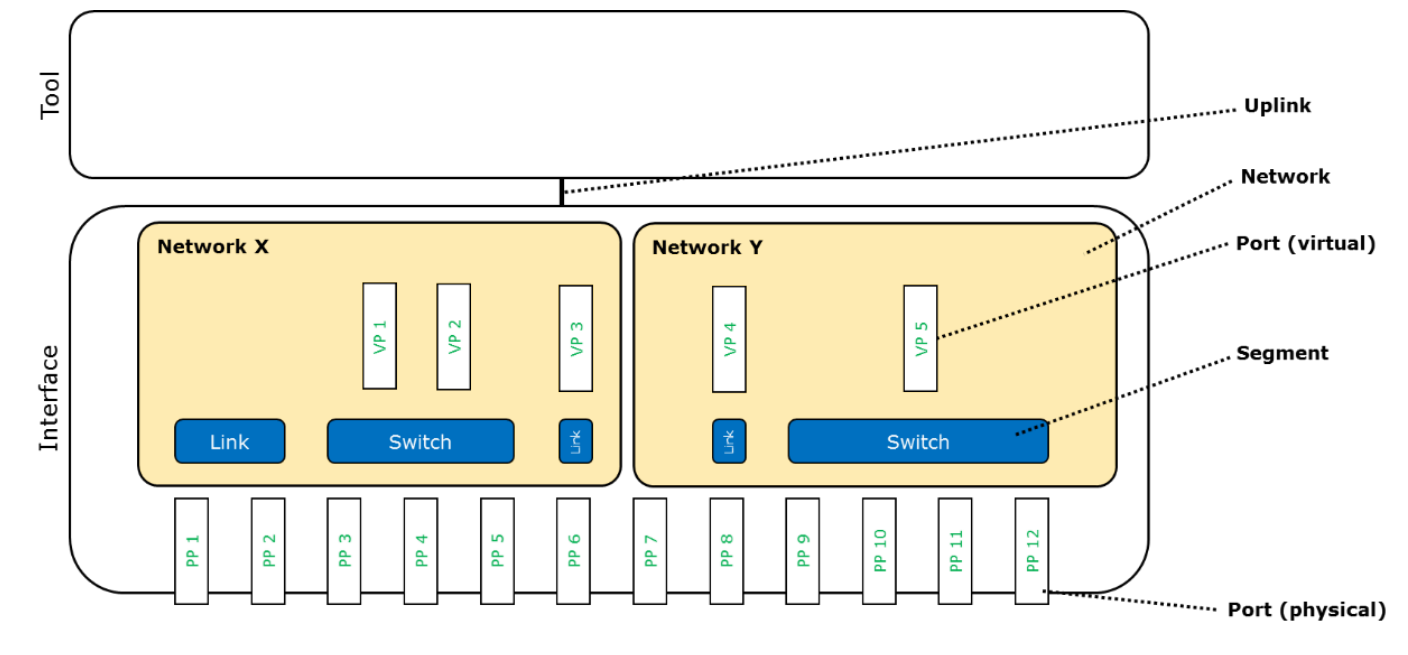
\includegraphics[scale=0.7]{pic/Snipaste_2021-10-29_09-46-43.png}
    \caption{术语实例}
    \label{fig:new_terms}
\end{figure}

\begin{enumerate}
    \item Port: 软件或硬件接入设备的入口,所以也分为物理端口和虚拟端口。CANoe 中仿真节点接入的就是虚拟端口。一个端口只能被一个 segment 包含。
    \item Segment: 分片是端口的组合。 必须至少创建一个分片并连接到一个物理端口。 每个分片都有一个唯一的名称,并且恰好分配给一个网络。 有两种类型的段可用:switch 和 link。 
    \begin{enumerate}
        \item switch segment: 提供 2 层交换机的功能。
        \item link segment: 完全透明地连接两个端口。 用于透明地转发以太网数据包和物理层的状态。Link segment 存在两种连接方式:TAP 和 直连。TAP 模式下,两个物理端口间有很小的延迟($\leq 6 \mu s$)。类似之前固件中提供的 MAC 旁路功能。
        直连模式适用于一个物理端口和虚拟端口间的连接。
    \end{enumerate}

    \item Network: 一个网络包括一个或多个分片。硬件设备中至少需要定义一个网络。
    \item Uplink: 设备和 CANoe PC 间的连接称为 uplink,可以通过配置 filter 减少传输给上位机的数据量。
\end{enumerate}

\subsubsection{概念变更}

\begin{figure}[ht]
    \centering
    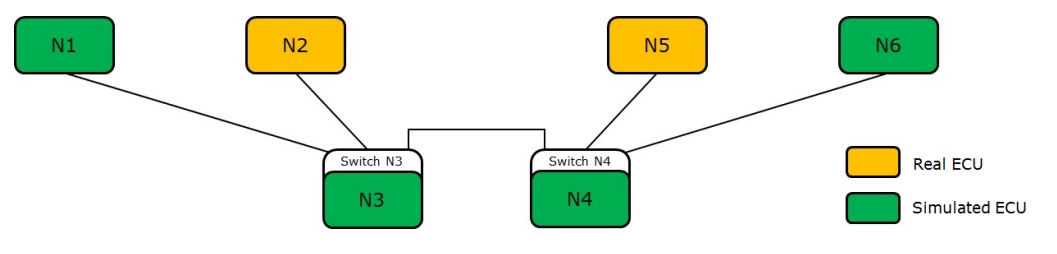
\includegraphics[scale=0.7]{pic/Snipaste_2021-10-29_14-37-48.png}
    \caption{拓扑实例}
    \label{fig:example_topology}
\end{figure}
图\ref{fig:example_topology} 包含两个复杂网络节点 \textbf{N3} 和 \textbf{N4},各自集成了一个 switch。
另外每个 switch 上连接了一个仿真节点 \textbf{N1} 和  \textbf{N6}。两个真实节点  \textbf{N2} 和  \textbf{N5}。

下图 \ref{fig:two_setup} 展示了固件版本 11.1 前后的实现方法。

\begin{figure}[ht]
    \centering
    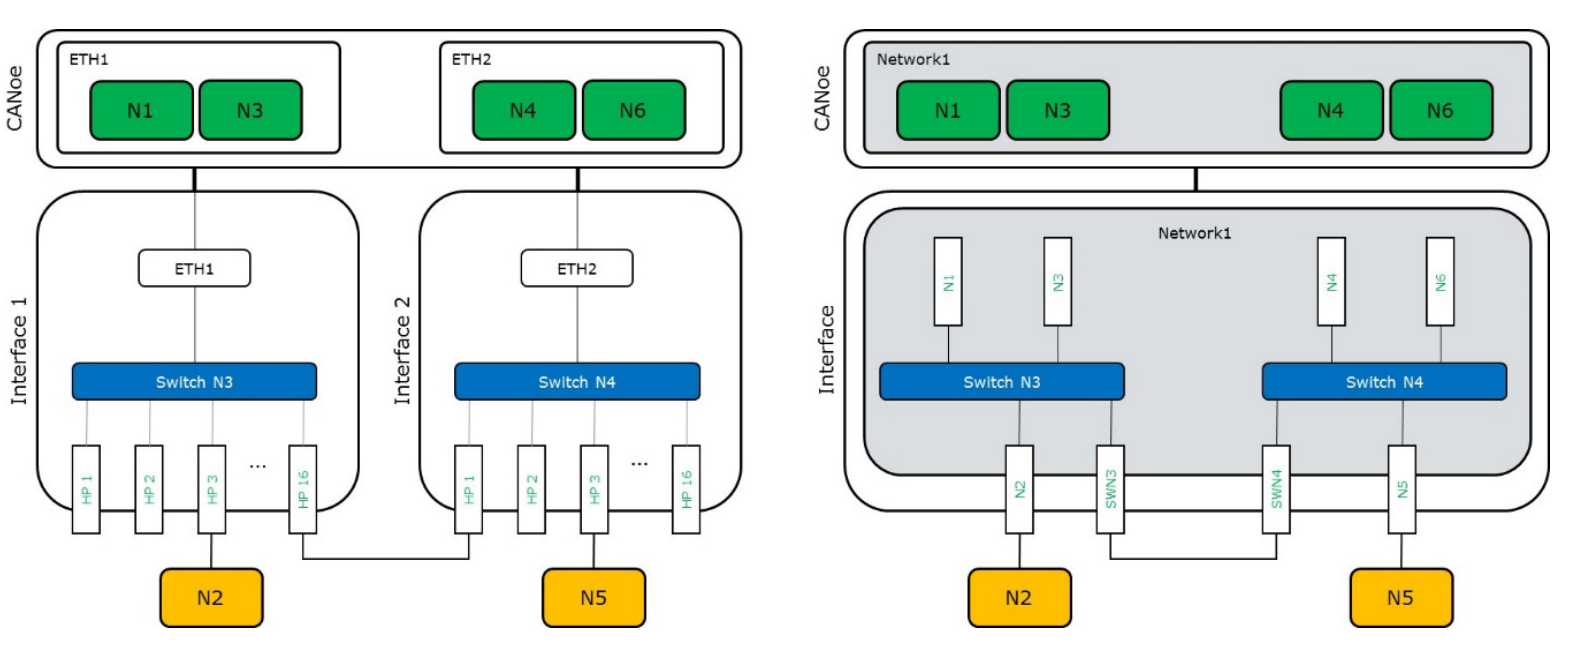
\includegraphics[scale=0.6]{pic/Snipaste_2021-10-29_14-42-44.png}
    \caption{ Simulation setup of the device firmware before version 11.1 vs. simulation setup of the device firmware from version 11.1}
    \label{fig:two_setup}
\end{figure}

之前版本中,一个设备仅能配置一个 switch 分片,因此,需要两个设备通过两个通道接入 CANoe。所以,在 CANoe 中需要配置两个 network。
之后版本中,允许自由配置分片。因此,可以配置两个 switch 分片,两个分片都分配在一个 network 中。因此,在 CANoe 中,仅需要配置一个 network。

\subsubsection{以太网包的收发方向}
设备接口接收到的以太网数据包总是标有 Rx 方向。 在这种情况下,数据包是由应用程序(例如 CANoe 模拟节点)生成还是来自真实网络无关紧要。
从接口发送到真实网络或模拟节点的数据包(例如,由于交换机段中的转发规则)被标记为 Tx 数据包。 
\begin{note}
    简单理解,新的方向,就是以硬件设备自身的角度考虑。从真实节点或仿真节点发给设备的都是 Rx 数据包,从设备发出去的都是 Tx 数据包。
\end{note}

\subsubsection{以太网硬件配置}
以太网硬件接口配置在 \textbf{Vector Hardware Config} 窗口中。如下图所示。
可以打开 \textbf{Ethernet Device Configuration}。

\begin{figure}[ht]
    \centering
    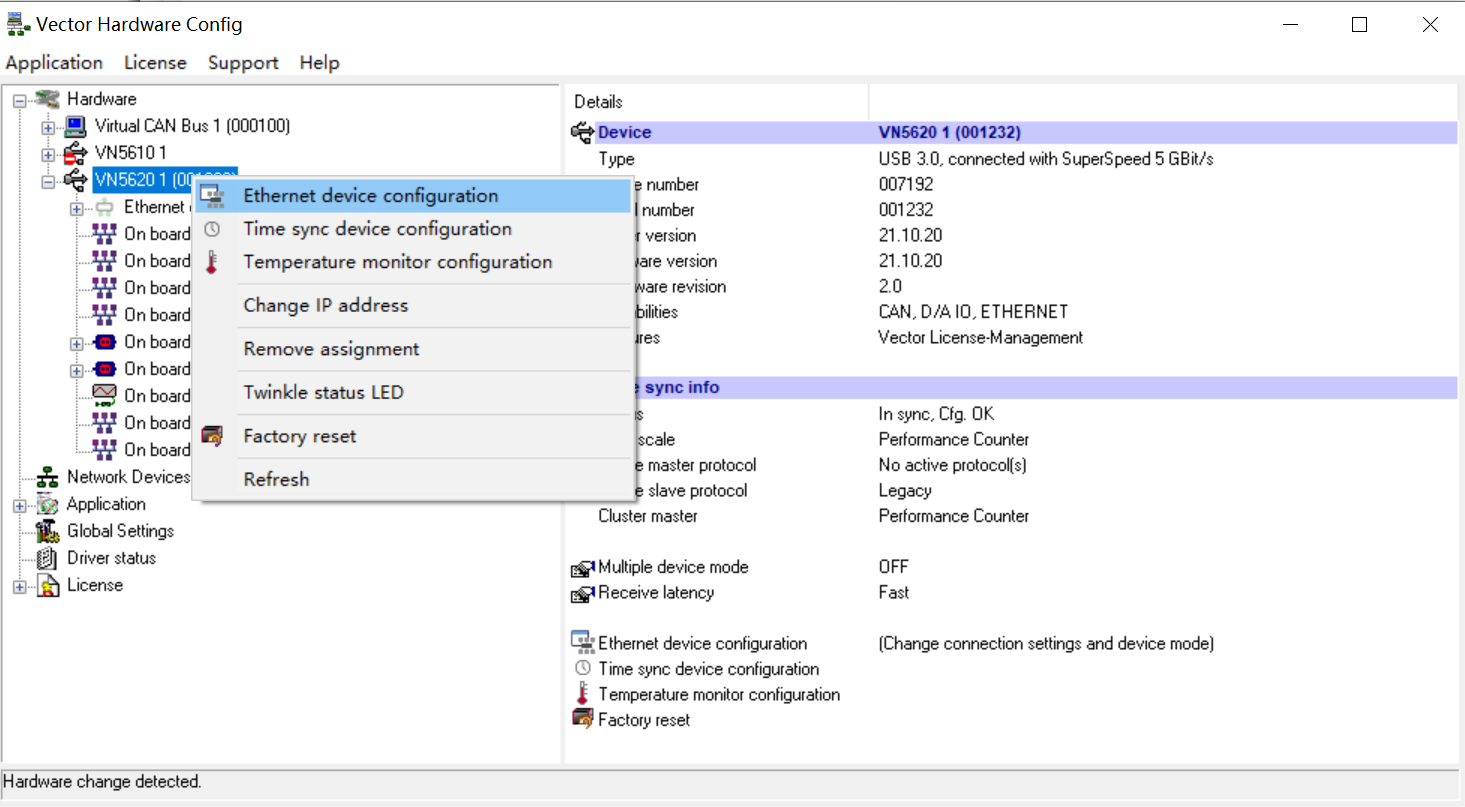
\includegraphics[scale=0.6]{pic/Snipaste_2021-10-29_15-00-01.png}
    \caption{ \textbf{Ethernet Device Configuration} 配置界面}
    \label{fig:Ethernet_Device_Configuration}
\end{figure}

下图\ref{fig:three_connect_ways}展示了三种连接方式,分别为:
\begin{itemize}
    \item 真实节点和仿真节点通过 switch 连接
    \item 真实节点和仿真节点直连
    \item 两个真实节点旁路连接,CANoe 作为检测
\end{itemize}

\begin{figure}[!ht]
    \centering
    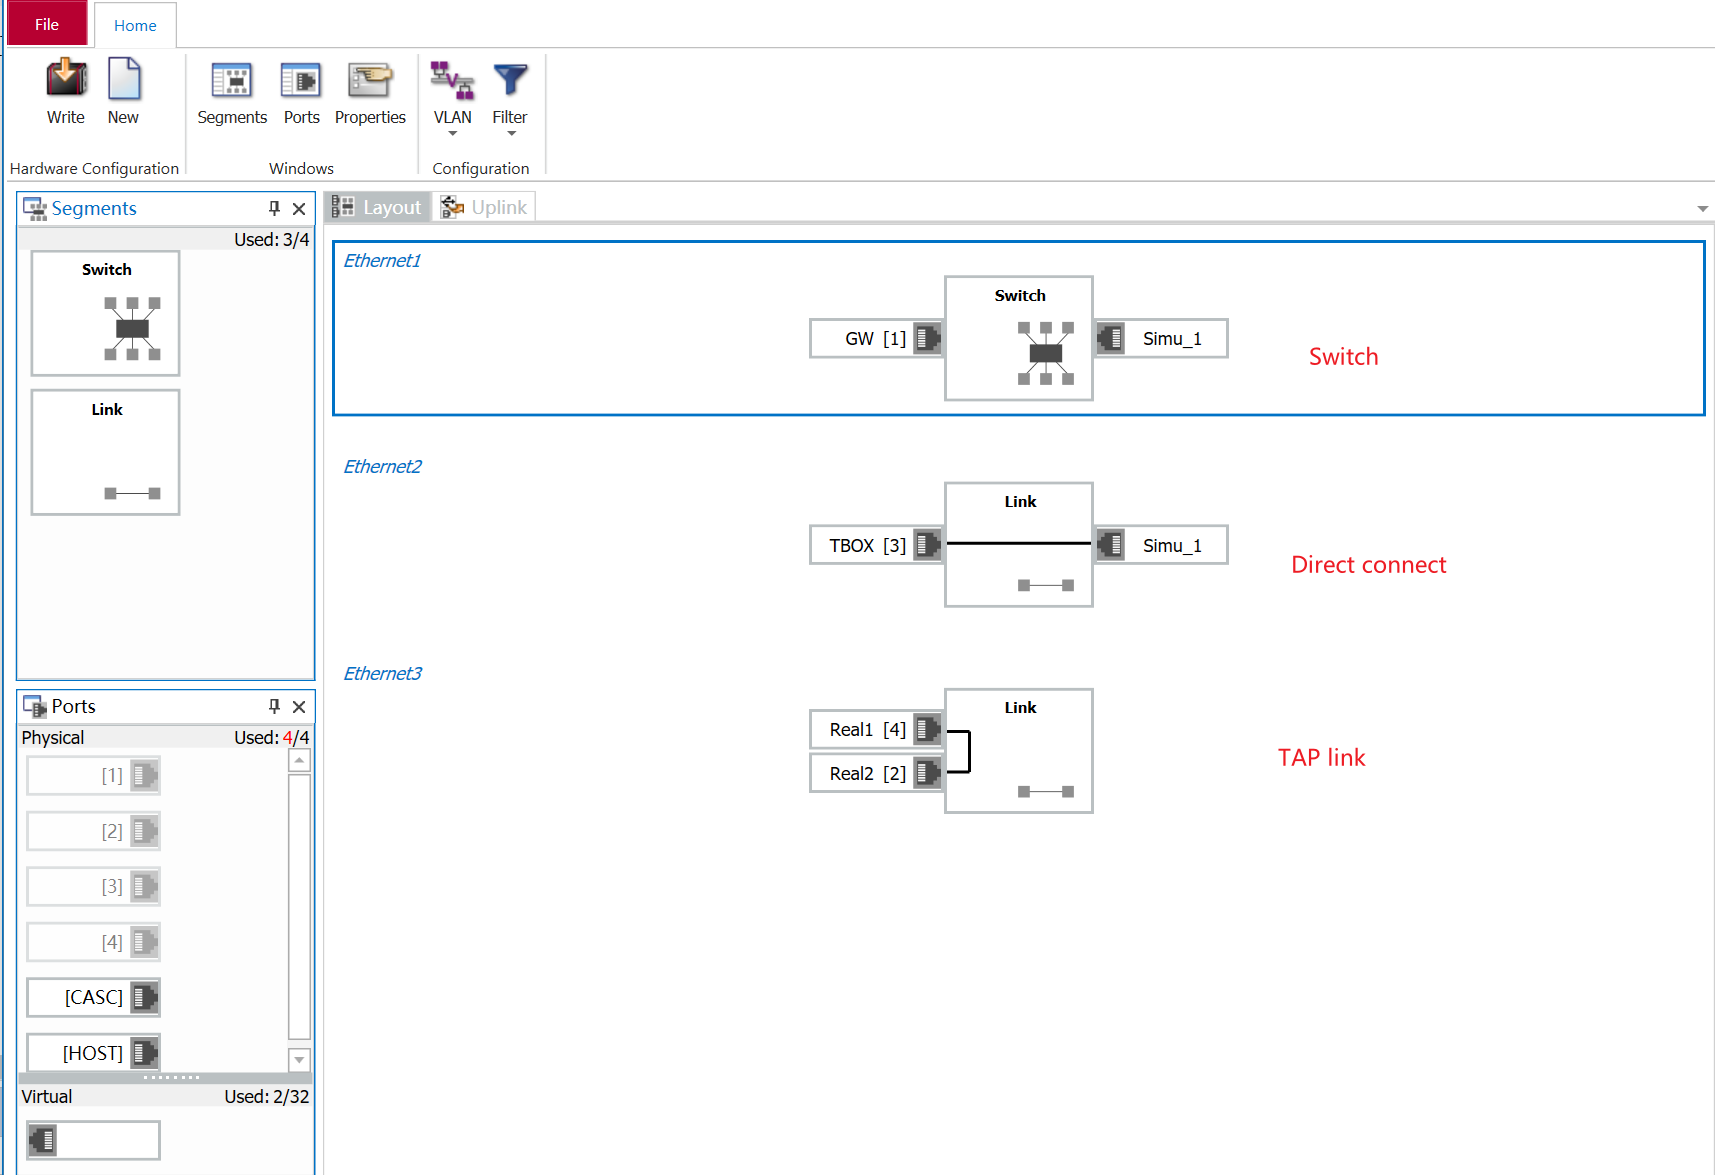
\includegraphics[scale=0.5]{pic/Snipaste_2021-10-29_15-06-06.png}
    \caption{三种连接方式}
    \label{fig:three_connect_ways}
\end{figure}

以第三种 TAP 连接方式为例,完成以上配置后,需要对以太网使用通道、通道和 network 映射、端口等进行详细配置。通道使用配置见下图\ref{fig:eth_channel_usage} \footnote{在实际使用中,仅需要使能 1 个通道,否则会报通道分配错误,详见图\ref{fig:eth_channel_usage_error}}。

\begin{figure}[ht]
    \centering
    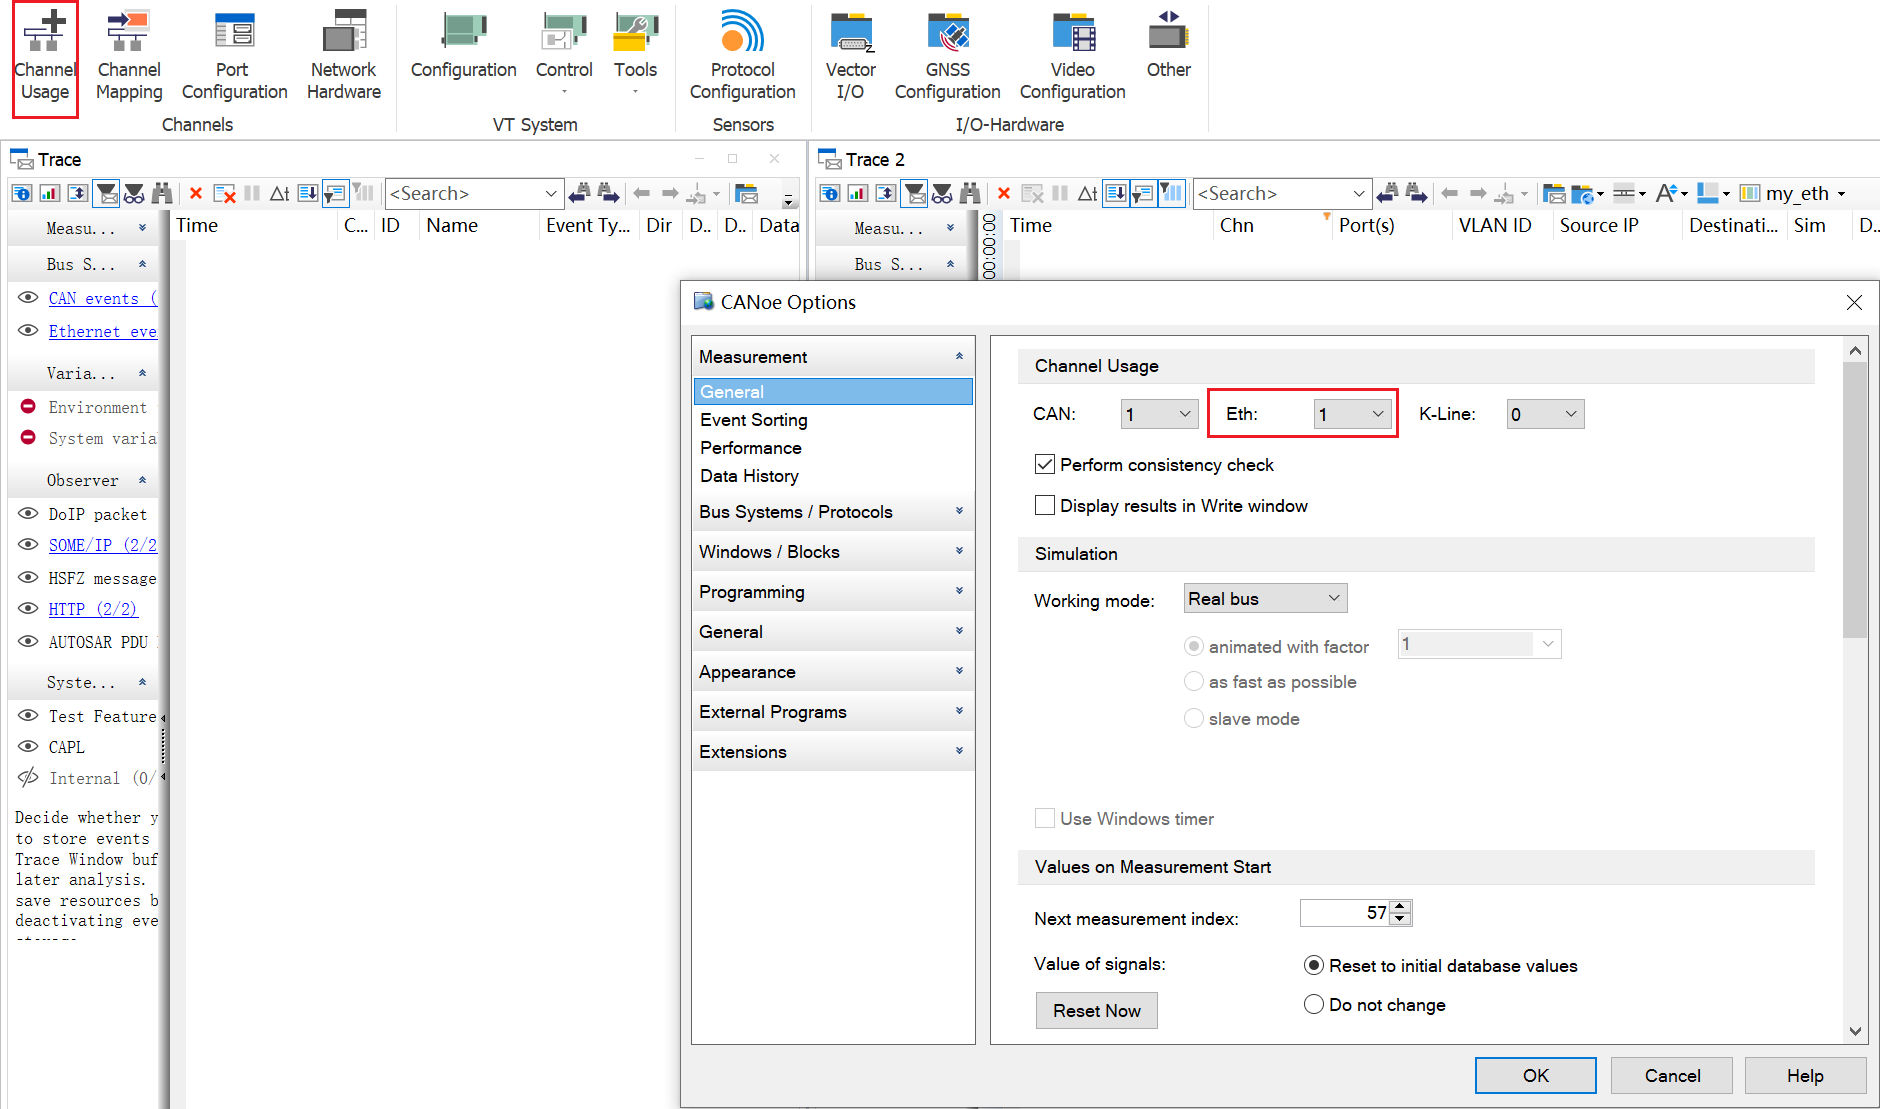
\includegraphics[scale=0.5]{pic/Snipaste_2021-10-29_15-18-52.png}
    \caption{以太网通道使用配置}
    \label{fig:eth_channel_usage}
\end{figure}

\begin{figure}[!ht]
    \centering
    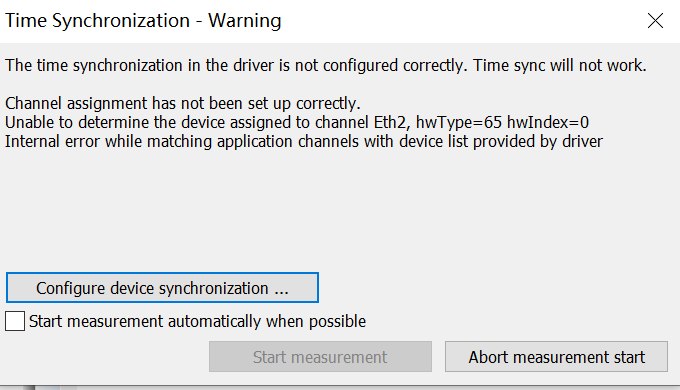
\includegraphics[scale=1]{pic/Snipaste_2021-10-29_15-22-58.png}
    \caption{以太网通道配置错误}
    \label{fig:eth_channel_usage_error}
\end{figure}

以太网通道映射,需要将以太网通道和 Simulation Setup 中定义的 Network 及 实际硬件配置的 network进行映射。详见图\ref{fig:eth_channel_mapping}。
\begin{figure}[!ht]
    \centering
    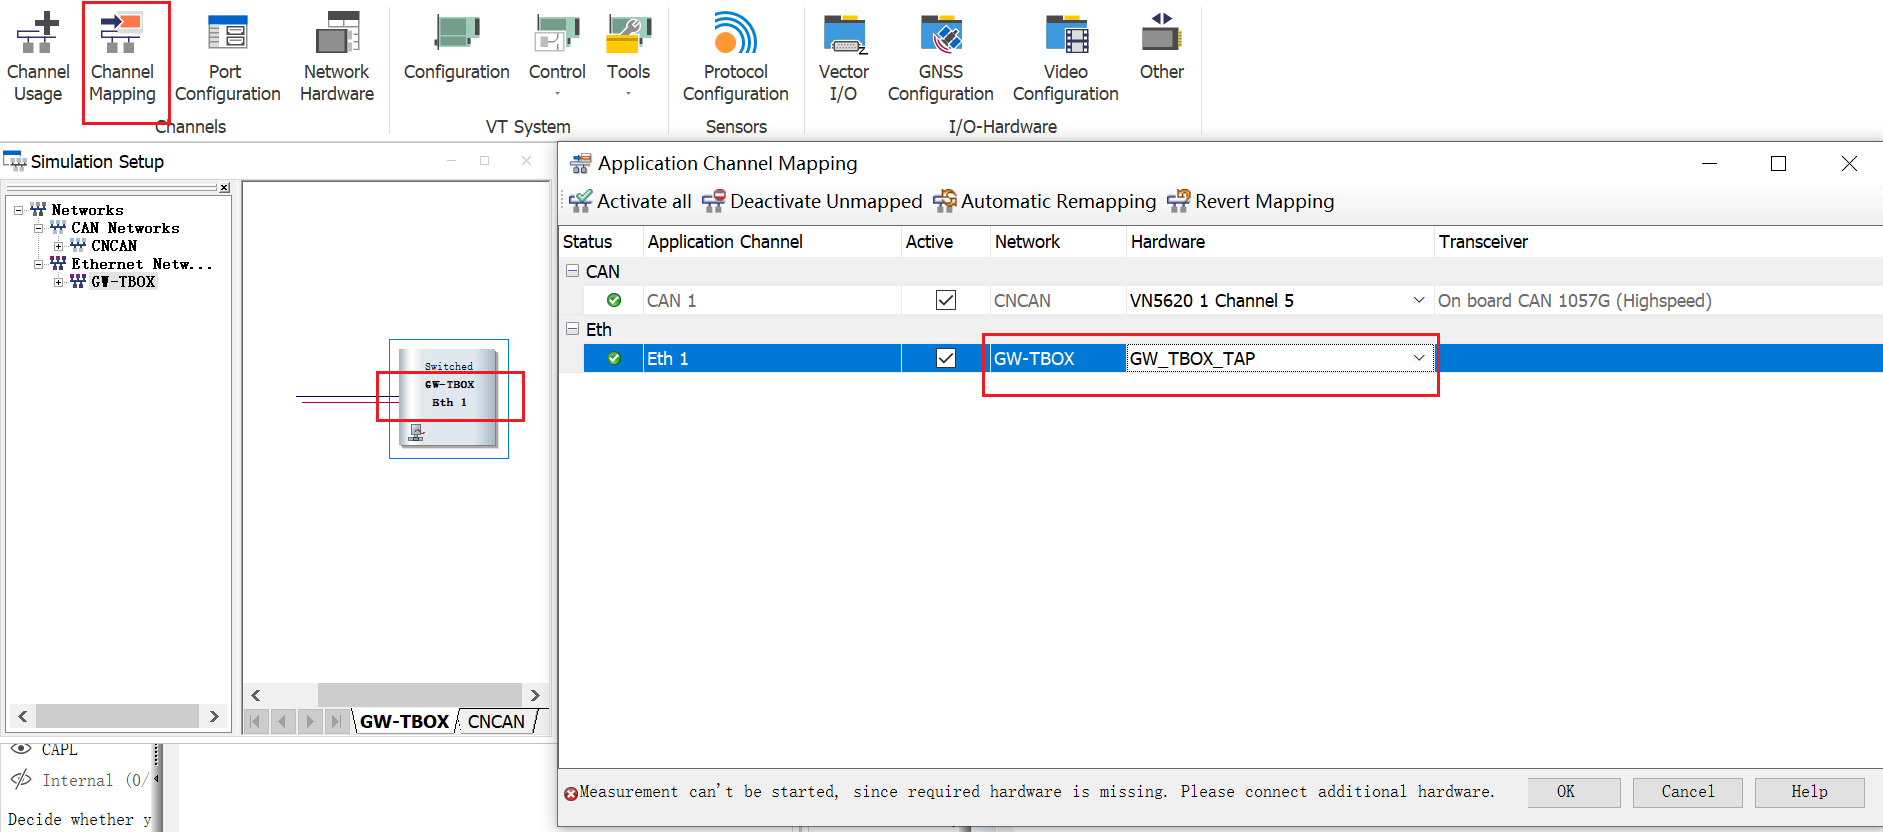
\includegraphics[scale=0.5]{pic/Snipaste_2021-10-29_15-25-55.png}
    \caption{以太网通道映射}
    \label{fig:eth_channel_mapping}
\end{figure}

最后,需要对端口状态进行配置,如进行激活等。详见图\ref{fig:port_Configuration}。
\begin{figure}[!ht]
    \centering
    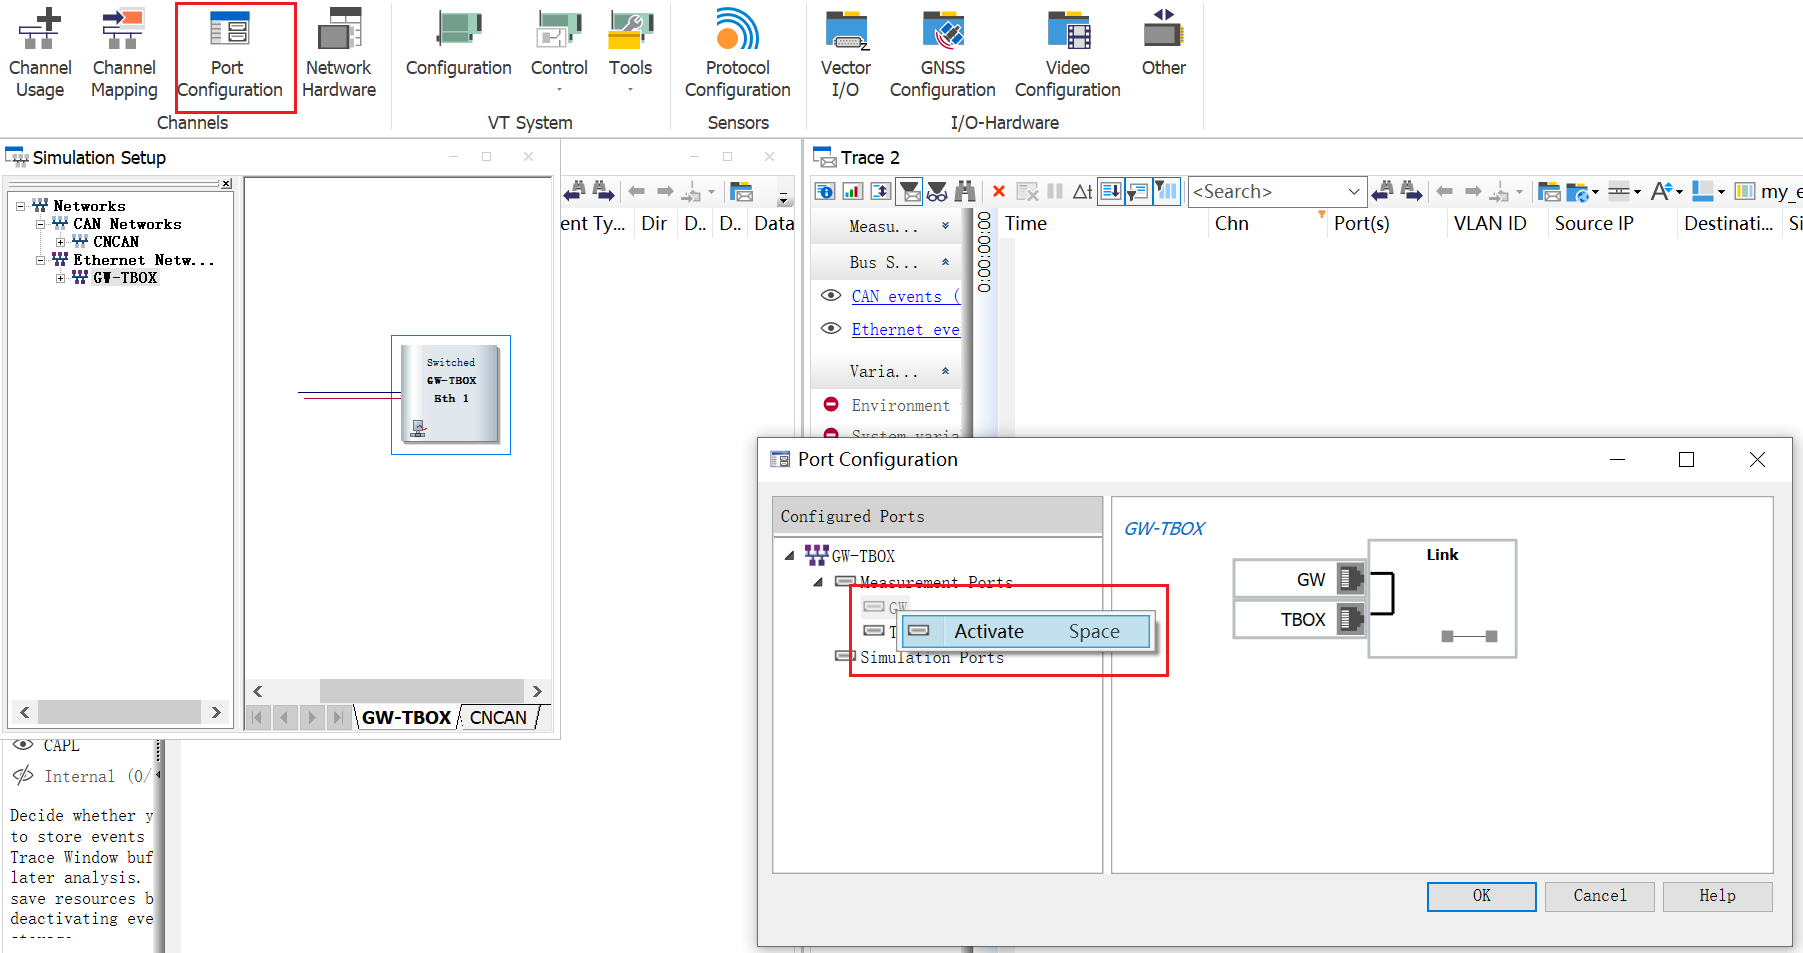
\includegraphics[scale=0.5]{pic/Snipaste_2021-10-29_15-29-21.png}
    \caption{以太网端口配置}
    \label{fig:port_Configuration}
\end{figure}

\subsection{TcpIp 协议栈配置}\label{sec:two_node_comm}
协议栈配置步骤中,主要对TCP/IP协议栈中的IP地址,mac 地址,VLAN 等配置。
以一个真实节点 GW 和一个仿真节点 ECU1 的通信为例,两节点通过 Link Direct 连接。对 ECU1 协议栈的配置如图\ref{fig:tcpip_Configuration}所示。

\begin{figure}[!ht]
    \centering
    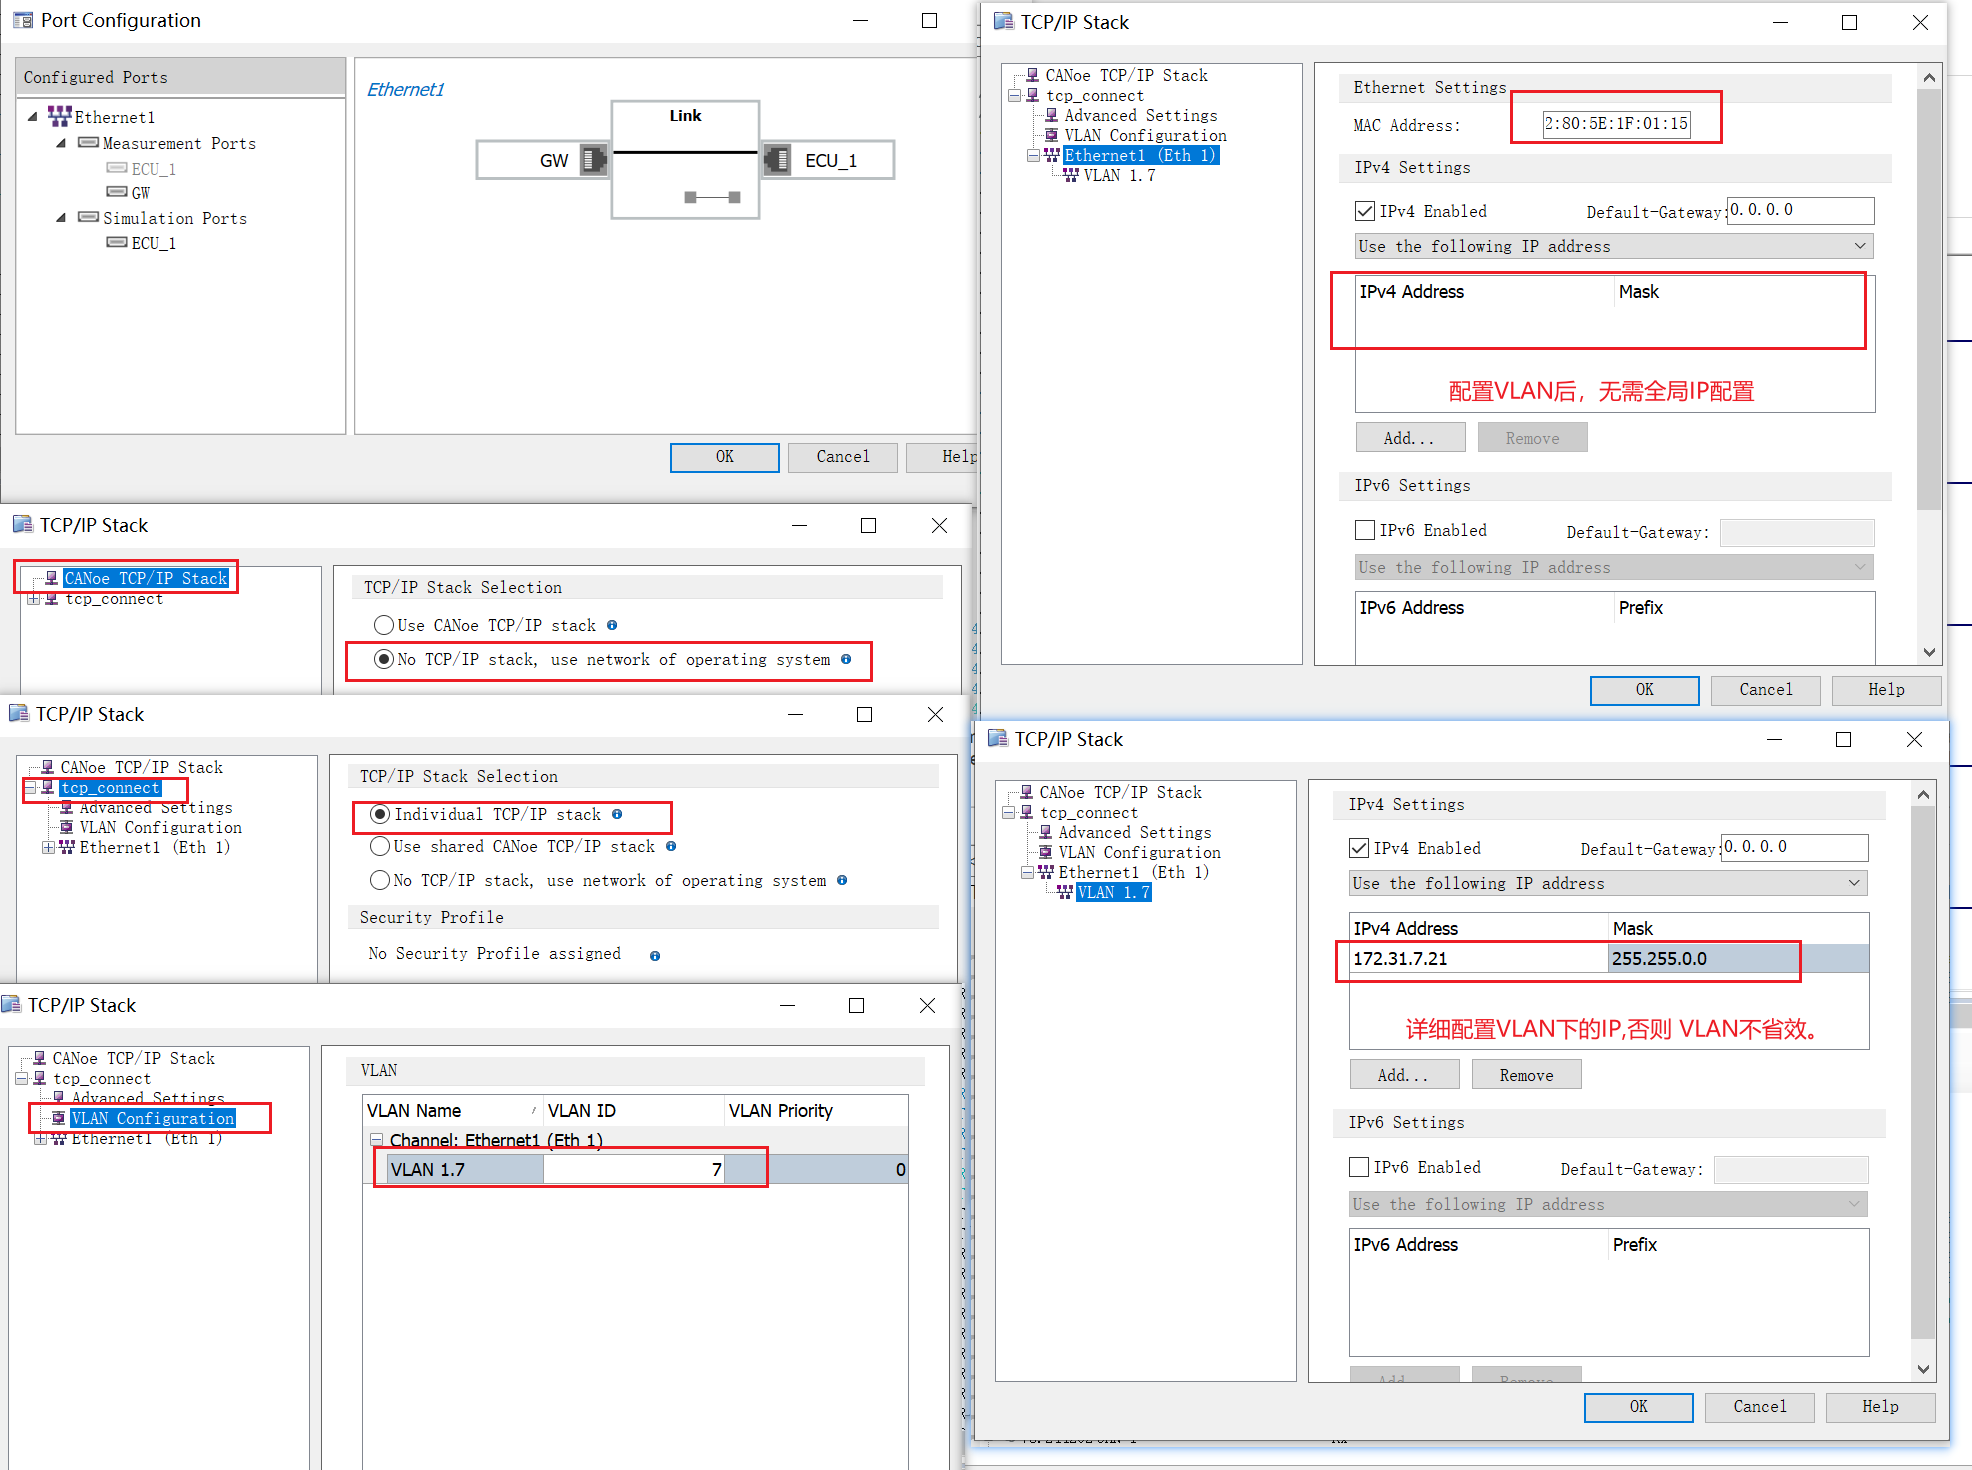
\includegraphics[scale=0.5]{pic/Snipaste_2021-10-29_16-08-23.png}
    \caption{以太网协议栈配置}
    \label{fig:tcpip_Configuration}
\end{figure}

\begin{note}
    当需要配置 VLAN 时,仿真节点协议栈中,一定要在 VLAN 详细配置中,添加对应的IP地址,否则,不能正常收发带正确 VLAN tag 的以太网帧,导致仿真结果出错。
\end{note}

\subsection{CAPL 仿真以太网节点}
以第\ref{sec:two_node_comm}节一个真实节点和一个仿真节点的通信为例,仿真节点的 CAPL 代码实现如下。
实现功能为:

\begin{enumerate}
    \item 启动后,发出 0x401 帧唤醒网络,并同时发出 0x459 帧,激活以太网DoIP功能。
    \item 等待 10s后,发起 TCP 握手,建立 TCP 连接。
    \item 等待 20s后,停发唤醒信号和以太网激活信号。
    \item 等待 60s后,网络应当休眠,重启计数器,循环上述过程。
\end{enumerate}
\begin{lstlisting}[language=C]




/*@!Encoding:936*/
// ---------------------------------------------------
// node global variables.
// ---------------------------------------------------
variables
{
  const int gMTU = 1500;                  // tcp mtu
  const dword gIPV4_STR_SIZE = 16;        // IPv4 string size
  const dword gINVALID_SOCKET = ~0;       // invalid socket constant
  dword gListenPort = 13400;              // port to send udp to.
  dword gClientSocket = gINVALID_SOCKET;  // client side: a demo client's socket.
  char gClientTcpBuffer[gMTU];            // tcp receive buffer of client
  //char gServerIpAddrStr[gIPV4_STR_SIZE] = "127.0.0.1"; // the IP of the server
  char gServerIpAddrStr[gIPV4_STR_SIZE] = "172.31.7.1"; // the IP of the server
  
  message 0x401 gWakeup_tbox;
  message 0x459 gDoipAct;
  msTimer gSendWakeTimer;
  msTimer gSendDoipActTimer;
  
  timer gStartTcpConnect;
  timer gStopWakeup;
  timer gRestartSimu;
  
  byte gStopWakeupFlag = 0;
  dword gTestNumber = 0;
}

on timer gSendWakeTimer
{
  gWakeup_tbox.byte(0) = 0x03;
  gWakeup_tbox.dlc = 1;
  output(gWakeup_tbox);
  if (0 == gStopWakeupFlag)
  {
    setTimer(gSendWakeTimer, 20);
  }
  
  
}

on timer gSendDoipActTimer
{
  gDoipAct.dlc = 8;
  gDoipAct.byte(4) = 0x10;
  output(gDoipAct);
  if (0 == gStopWakeupFlag)
  {
    setTimer(gSendDoipActTimer, 100);
  }
  
  
}

on timer gStartTcpConnect
{
  clientConnect();
}


on timer gStopWakeup
{
  gStopWakeupFlag = 1;
}

on timer gRestartSimu
{
  gTestNumber ++;
  
  write("*******************************TEST NUMBER %d **********************************************",gTestNumber);
  gStopWakeupFlag = 0;
  setTimer(gSendWakeTimer, 20);
  setTimer(gSendDoipActTimer, 100);
  setTimer(gStartTcpConnect, 10);
  setTimer(gStopWakeup, 20);
  //clientConnect();
  setTimer(gRestartSimu,60);
}
// ---------------------------------------------------
// Interaction: Client connects to server
// ---------------------------------------------------
on key 'c'
{
  clientConnect();
}

// ---------------------------------------------------
// Interaction: Client disconnects from server.
// ---------------------------------------------------
on key 'd'
{
  clientDisconnect();
}

// ---------------------------------------------------
// Interaction: Client sends a request to the server
// ---------------------------------------------------
on key 's'
{
  clientSendRequest();
}

// ---------------------------------------------------
// Interaction: Stop measurement
// ---------------------------------------------------
on key 'q'
{
  stop();
}

// ---------------------------------------------------
// Connection operation completes
// ---------------------------------------------------
void OnTcpConnect( dword socket, long result)
{
  writeLineEx(1, 1, " [ C: OnTcpConnect called. (result: %d)]", result);
  if (result == 0)
  {
    if (socket == gClientSocket)
    {
      write("C: Client connected to server done. (socket: %d, result: %d)", socket, result);
      clientSendRequest();
      startReceive(gClientSocket, gClientTcpBuffer);
    }
  }
}

// ---------------------------------------------------
// When asynchronous TcpSend completes...
// ---------------------------------------------------
void OnTcpSend( dword socket, long result, char buffer[], dword size)
{
  writeLineEx(1, 1, " [ C: OnTcpSend called. (result: %d)]", result);
  if (result == 0)
  {
    if (socket != gINVALID_SOCKET)
    {
      if (socket == gClientSocket)
      {
        write("C: Client sent %d bytes to server done. (socket %d, result: %d)", size, socket, result);
      }
    }
  }
}

// ---------------------------------------------------
// When receiving data on socket...
// ---------------------------------------------------
void OnTcpReceive( dword socket, long result, dword address, dword port, char buffer[], dword size)
{
  dword i;
  byte sendDiagData[14] = {
    0x02, 0xfd, 0x80, 0x01, 0x00,0x00,0x00,0x06,  0x0f,0x00,0x10,0x00, 0x10, 0x03
  };
  writeLineEx(1, 1, " [ C: OnTcpReceive called. (result: %d) ]", result);
  if (result == 0)
  {
    if (socket == gClientSocket)
    {
      // client receives from server...
      write("C: Client received %d bytes from server: %s (result: %d)", size, buffer, result);
      
//      for(i=0; i<size;i++)
//      {
//        write("%x",buffer[i]);
//        
//      }
      // check server's answer...
      if (strstr(buffer, "WELCOME") >= 0)
      {
        write("C: Server told us WELCOME. Connection established.");
      }
      else if (strstr(buffer, "ANSWER") >= 0)
      {
        write("C: Received server answer: %s", buffer);
      }
      
      startReceive(gClientSocket, gClientTcpBuffer);
      if(size == 21)
      {
        sendTcpData(gClientSocket, sendDiagData, 14);
      }
      else if(size == 18)
      {
        clientDisconnect();
      }
      // continue receiving data on valid socket.
      //startReceive(gClientSocket, gClientTcpBuffer);
      // show menu...
      showMenu(1);
    }
    else if (socket != gINVALID_SOCKET)
    {
      writeLineEx(1, 3, " [ C: UNIMPLEMENTED: Received %d bytes on socket %d from 0x%x:%d with data: %s (result: %d) ]", size, socket, address, port, buffer, result);
    }
  }
}

// ---------------------------------------------------
// TCP socket receives a close notification
// ( remote closed )
// ---------------------------------------------------
void OnTcpClose( dword socket, long result)
{
  if (socket == gClientSocket)
  {
    TcpClose(gClientSocket);
    gClientSocket = gINVALID_SOCKET;
    writeLineEx(1, 1, " [ C: OnTcpClose called. (socket: %d, result: %d) ]", socket, result);
    showMenu(0);
  }
}

// ---------------------------------------------------
// connect a client...
// ---------------------------------------------------
void clientConnect()
{
  dword result;
  if (gClientSocket != gINVALID_SOCKET)
  {
    writeLineEx(1, 2, " [ C: The client is already connected. ]");
    return;
  }
  writeLineEx(1, 1, " [ C: DEMO connecting one client... ]");
  gClientSocket = TcpOpen( 0, 0 );
  if (gClientSocket == gINVALID_SOCKET)
  {
    writeLineEx(1, 3, " [ C: TcpOpen: FAILED. ]");
  }
  else
  {
    result = TcpConnect( gClientSocket, IpGetAddressAsNumber(gServerIpAddrStr), gListenPort );
    if ( result == -1 )
    {
      result = IpGetLastSocketError(gClientSocket);
      if (result != 10035)
      {
        writeLineEx( 1, 3, " [ C: TcpConnect for client failed with error %d ]", result );
      }
    }
    else
    {
      writeLineEx(1, 3, " [ C: TcpConnect for client failed with error %d ]", result);
    };
    // => Connection established in callback OnTcpConnect...
  }
}

// ---------------------------------------------------
// client disconnects...
// ---------------------------------------------------
void clientDisconnect()
{
  if (gClientSocket != gINVALID_SOCKET)
  {
    write("C: Disconnecting from server. (socket %d)", gClientSocket);
    TcpClose(gClientSocket);
    gClientSocket = gINVALID_SOCKET;
    //showMenu(0);
  }
}

// ---------------------------------------------------
// client sends a request to server.
// ---------------------------------------------------
void clientSendRequest()
{
  // if client is connected...
  byte sendData[19] = {
    0x02, 0xfd, 0x00, 0x05, 0x00, 0x00, 0x00,0x0b,0x0f,0x00,0x00,0x00,0x00,0x00,0x00,0x00,0x00,0x00,0x00
  };
  
  if (gClientSocket != gINVALID_SOCKET)
  {
    write("C: Sending data to server. (socket %d)", gClientSocket);
    sendTcpData(gClientSocket, sendData, 19);
    //sendTcpData(gClientSocket, sendData, 14);
  }
  
}

// ---------------------------------------------------
// show a little write menu to let you know what you can do next.
// ---------------------------------------------------
void showMenu(int connected)
{
//  write("--------------[MENU]--------------------");
//  if (!connected)
//  {
//    write("- Press 'c' to connect client ...");
//  }
//  else
//  {
//    write("- Press 's' to send message to server...");
//    write("- Press 'd' to disconnect from server...");
//    write("- Press 'x' to let server disconnect client...");
//  }
//  write("- Press 'q' to stop measurement...");
//  write("----------------------------------------");
}

// ---------------------------------------------------
// send tcp data.
// ---------------------------------------------------
void sendTcpData( dword socket, byte data[], dword size )
{
 long result;
  //dword size;
  //size = elcount(data);
  result = TcpSend(socket, data, size);
  if (result == 0)
  {
    // sending took place immediately.
    //writeLineEx(1, 1, " [ C: Synchronous sending: '%s' on socket %d ]", data, socket);
    //OnTcpSend(socket, result, data, size); // trigger callback manually
  }
  else
  {
    if (result == -1)
    {
      result = IpGetLastSocketError(socket);
      if (result == 997)
      {
        // sending is done asynchronously.
       // writeLineEx(1, 1, " [ C: Asynchronous sending: '%s' on socket %d ]", data, socket);
        // => OnTcpSend is called when done sending.
      }
      else
      {
        writeLineEx( 1, 3, " [ C: sendTcpData: Error sending data. (%d) ]", result);
      }
    }
    else
    {
      writeLineEx( 1, 3, " [ C: sendTcpData: Error sending data. (%d) ]", result);
    }
  }
}
on start
{
  //showMenu(0);
  
  
  setTimer(gSendWakeTimer, 20);
  setTimer(gSendDoipActTimer, 100);
  setTimer(gStartTcpConnect, 10);
  setTimer(gStopWakeup, 20);
  //clientConnect();
  setTimer(gRestartSimu,60);
  
}

// ---------------------------------------------------
// start receiving on given socket into given buffer.
// ---------------------------------------------------
void startReceive ( dword socket, char buffer[] )
{
  long result;
  result = TcpReceive( socket, buffer, elcount(buffer) );
  if (result == -1)
  {
    result = IpGetLastSocketError(socket);
    if (result != 997) // not asynchronous
    {
      // failure
      writeLineEx( 1, 3, "S: TcpReceive error %d", result);
    }
  }
  else if (result != 0) // synchronous sending failed
  {
    // failure
    writeLineEx( 1, 3, "S: TcpReceive error %d", result);
  }
}

\end{lstlisting}
